% Options for packages loaded elsewhere
\PassOptionsToPackage{unicode}{hyperref}
\PassOptionsToPackage{hyphens}{url}
\PassOptionsToPackage{dvipsnames,svgnames,x11names}{xcolor}
%
\documentclass[
  letterpaper,
  DIV=11,
  numbers=noendperiod]{scrartcl}

\usepackage{amsmath,amssymb}
\usepackage{lmodern}
\usepackage{iftex}
\ifPDFTeX
  \usepackage[T1]{fontenc}
  \usepackage[utf8]{inputenc}
  \usepackage{textcomp} % provide euro and other symbols
\else % if luatex or xetex
  \usepackage{unicode-math}
  \defaultfontfeatures{Scale=MatchLowercase}
  \defaultfontfeatures[\rmfamily]{Ligatures=TeX,Scale=1}
\fi
% Use upquote if available, for straight quotes in verbatim environments
\IfFileExists{upquote.sty}{\usepackage{upquote}}{}
\IfFileExists{microtype.sty}{% use microtype if available
  \usepackage[]{microtype}
  \UseMicrotypeSet[protrusion]{basicmath} % disable protrusion for tt fonts
}{}
\makeatletter
\@ifundefined{KOMAClassName}{% if non-KOMA class
  \IfFileExists{parskip.sty}{%
    \usepackage{parskip}
  }{% else
    \setlength{\parindent}{0pt}
    \setlength{\parskip}{6pt plus 2pt minus 1pt}}
}{% if KOMA class
  \KOMAoptions{parskip=half}}
\makeatother
\usepackage{xcolor}
\setlength{\emergencystretch}{3em} % prevent overfull lines
\setcounter{secnumdepth}{-\maxdimen} % remove section numbering
% Make \paragraph and \subparagraph free-standing
\ifx\paragraph\undefined\else
  \let\oldparagraph\paragraph
  \renewcommand{\paragraph}[1]{\oldparagraph{#1}\mbox{}}
\fi
\ifx\subparagraph\undefined\else
  \let\oldsubparagraph\subparagraph
  \renewcommand{\subparagraph}[1]{\oldsubparagraph{#1}\mbox{}}
\fi

\usepackage{color}
\usepackage{fancyvrb}
\newcommand{\VerbBar}{|}
\newcommand{\VERB}{\Verb[commandchars=\\\{\}]}
\DefineVerbatimEnvironment{Highlighting}{Verbatim}{commandchars=\\\{\}}
% Add ',fontsize=\small' for more characters per line
\usepackage{framed}
\definecolor{shadecolor}{RGB}{241,243,245}
\newenvironment{Shaded}{\begin{snugshade}}{\end{snugshade}}
\newcommand{\AlertTok}[1]{\textcolor[rgb]{0.68,0.00,0.00}{#1}}
\newcommand{\AnnotationTok}[1]{\textcolor[rgb]{0.37,0.37,0.37}{#1}}
\newcommand{\AttributeTok}[1]{\textcolor[rgb]{0.40,0.45,0.13}{#1}}
\newcommand{\BaseNTok}[1]{\textcolor[rgb]{0.68,0.00,0.00}{#1}}
\newcommand{\BuiltInTok}[1]{\textcolor[rgb]{0.00,0.23,0.31}{#1}}
\newcommand{\CharTok}[1]{\textcolor[rgb]{0.13,0.47,0.30}{#1}}
\newcommand{\CommentTok}[1]{\textcolor[rgb]{0.37,0.37,0.37}{#1}}
\newcommand{\CommentVarTok}[1]{\textcolor[rgb]{0.37,0.37,0.37}{\textit{#1}}}
\newcommand{\ConstantTok}[1]{\textcolor[rgb]{0.56,0.35,0.01}{#1}}
\newcommand{\ControlFlowTok}[1]{\textcolor[rgb]{0.00,0.23,0.31}{#1}}
\newcommand{\DataTypeTok}[1]{\textcolor[rgb]{0.68,0.00,0.00}{#1}}
\newcommand{\DecValTok}[1]{\textcolor[rgb]{0.68,0.00,0.00}{#1}}
\newcommand{\DocumentationTok}[1]{\textcolor[rgb]{0.37,0.37,0.37}{\textit{#1}}}
\newcommand{\ErrorTok}[1]{\textcolor[rgb]{0.68,0.00,0.00}{#1}}
\newcommand{\ExtensionTok}[1]{\textcolor[rgb]{0.00,0.23,0.31}{#1}}
\newcommand{\FloatTok}[1]{\textcolor[rgb]{0.68,0.00,0.00}{#1}}
\newcommand{\FunctionTok}[1]{\textcolor[rgb]{0.28,0.35,0.67}{#1}}
\newcommand{\ImportTok}[1]{\textcolor[rgb]{0.00,0.46,0.62}{#1}}
\newcommand{\InformationTok}[1]{\textcolor[rgb]{0.37,0.37,0.37}{#1}}
\newcommand{\KeywordTok}[1]{\textcolor[rgb]{0.00,0.23,0.31}{#1}}
\newcommand{\NormalTok}[1]{\textcolor[rgb]{0.00,0.23,0.31}{#1}}
\newcommand{\OperatorTok}[1]{\textcolor[rgb]{0.37,0.37,0.37}{#1}}
\newcommand{\OtherTok}[1]{\textcolor[rgb]{0.00,0.23,0.31}{#1}}
\newcommand{\PreprocessorTok}[1]{\textcolor[rgb]{0.68,0.00,0.00}{#1}}
\newcommand{\RegionMarkerTok}[1]{\textcolor[rgb]{0.00,0.23,0.31}{#1}}
\newcommand{\SpecialCharTok}[1]{\textcolor[rgb]{0.37,0.37,0.37}{#1}}
\newcommand{\SpecialStringTok}[1]{\textcolor[rgb]{0.13,0.47,0.30}{#1}}
\newcommand{\StringTok}[1]{\textcolor[rgb]{0.13,0.47,0.30}{#1}}
\newcommand{\VariableTok}[1]{\textcolor[rgb]{0.07,0.07,0.07}{#1}}
\newcommand{\VerbatimStringTok}[1]{\textcolor[rgb]{0.13,0.47,0.30}{#1}}
\newcommand{\WarningTok}[1]{\textcolor[rgb]{0.37,0.37,0.37}{\textit{#1}}}

\providecommand{\tightlist}{%
  \setlength{\itemsep}{0pt}\setlength{\parskip}{0pt}}\usepackage{longtable,booktabs,array}
\usepackage{calc} % for calculating minipage widths
% Correct order of tables after \paragraph or \subparagraph
\usepackage{etoolbox}
\makeatletter
\patchcmd\longtable{\par}{\if@noskipsec\mbox{}\fi\par}{}{}
\makeatother
% Allow footnotes in longtable head/foot
\IfFileExists{footnotehyper.sty}{\usepackage{footnotehyper}}{\usepackage{footnote}}
\makesavenoteenv{longtable}
\usepackage{graphicx}
\makeatletter
\def\maxwidth{\ifdim\Gin@nat@width>\linewidth\linewidth\else\Gin@nat@width\fi}
\def\maxheight{\ifdim\Gin@nat@height>\textheight\textheight\else\Gin@nat@height\fi}
\makeatother
% Scale images if necessary, so that they will not overflow the page
% margins by default, and it is still possible to overwrite the defaults
% using explicit options in \includegraphics[width, height, ...]{}
\setkeys{Gin}{width=\maxwidth,height=\maxheight,keepaspectratio}
% Set default figure placement to htbp
\makeatletter
\def\fps@figure{htbp}
\makeatother
\newlength{\cslhangindent}
\setlength{\cslhangindent}{1.5em}
\newlength{\csllabelwidth}
\setlength{\csllabelwidth}{3em}
\newlength{\cslentryspacingunit} % times entry-spacing
\setlength{\cslentryspacingunit}{\parskip}
\newenvironment{CSLReferences}[2] % #1 hanging-ident, #2 entry spacing
 {% don't indent paragraphs
  \setlength{\parindent}{0pt}
  % turn on hanging indent if param 1 is 1
  \ifodd #1
  \let\oldpar\par
  \def\par{\hangindent=\cslhangindent\oldpar}
  \fi
  % set entry spacing
  \setlength{\parskip}{#2\cslentryspacingunit}
 }%
 {}
\usepackage{calc}
\newcommand{\CSLBlock}[1]{#1\hfill\break}
\newcommand{\CSLLeftMargin}[1]{\parbox[t]{\csllabelwidth}{#1}}
\newcommand{\CSLRightInline}[1]{\parbox[t]{\linewidth - \csllabelwidth}{#1}\break}
\newcommand{\CSLIndent}[1]{\hspace{\cslhangindent}#1}

\KOMAoption{captions}{tableheading}
\makeatletter
\@ifpackageloaded{tcolorbox}{}{\usepackage[many]{tcolorbox}}
\@ifpackageloaded{fontawesome5}{}{\usepackage{fontawesome5}}
\definecolor{quarto-callout-color}{HTML}{909090}
\definecolor{quarto-callout-note-color}{HTML}{0758E5}
\definecolor{quarto-callout-important-color}{HTML}{CC1914}
\definecolor{quarto-callout-warning-color}{HTML}{EB9113}
\definecolor{quarto-callout-tip-color}{HTML}{00A047}
\definecolor{quarto-callout-caution-color}{HTML}{FC5300}
\definecolor{quarto-callout-color-frame}{HTML}{acacac}
\definecolor{quarto-callout-note-color-frame}{HTML}{4582ec}
\definecolor{quarto-callout-important-color-frame}{HTML}{d9534f}
\definecolor{quarto-callout-warning-color-frame}{HTML}{f0ad4e}
\definecolor{quarto-callout-tip-color-frame}{HTML}{02b875}
\definecolor{quarto-callout-caution-color-frame}{HTML}{fd7e14}
\makeatother
\makeatletter
\makeatother
\makeatletter
\makeatother
\makeatletter
\@ifpackageloaded{caption}{}{\usepackage{caption}}
\AtBeginDocument{%
\ifdefined\contentsname
  \renewcommand*\contentsname{Table of contents}
\else
  \newcommand\contentsname{Table of contents}
\fi
\ifdefined\listfigurename
  \renewcommand*\listfigurename{List of Figures}
\else
  \newcommand\listfigurename{List of Figures}
\fi
\ifdefined\listtablename
  \renewcommand*\listtablename{List of Tables}
\else
  \newcommand\listtablename{List of Tables}
\fi
\ifdefined\figurename
  \renewcommand*\figurename{Figure}
\else
  \newcommand\figurename{Figure}
\fi
\ifdefined\tablename
  \renewcommand*\tablename{Table}
\else
  \newcommand\tablename{Table}
\fi
}
\@ifpackageloaded{float}{}{\usepackage{float}}
\floatstyle{ruled}
\@ifundefined{c@chapter}{\newfloat{codelisting}{h}{lop}}{\newfloat{codelisting}{h}{lop}[chapter]}
\floatname{codelisting}{Listing}
\newcommand*\listoflistings{\listof{codelisting}{List of Listings}}
\makeatother
\makeatletter
\@ifpackageloaded{caption}{}{\usepackage{caption}}
\@ifpackageloaded{subcaption}{}{\usepackage{subcaption}}
\makeatother
\makeatletter
\@ifpackageloaded{tcolorbox}{}{\usepackage[many]{tcolorbox}}
\makeatother
\makeatletter
\@ifundefined{shadecolor}{\definecolor{shadecolor}{rgb}{.97, .97, .97}}
\makeatother
\makeatletter
\makeatother
\ifLuaTeX
  \usepackage{selnolig}  % disable illegal ligatures
\fi
\IfFileExists{bookmark.sty}{\usepackage{bookmark}}{\usepackage{hyperref}}
\IfFileExists{xurl.sty}{\usepackage{xurl}}{} % add URL line breaks if available
\urlstyle{same} % disable monospaced font for URLs
\hypersetup{
  pdftitle={GEO 3/446 Exercise \#2},
  pdfauthor={C. Scott Smith, PhD AICP (Instructor)},
  colorlinks=true,
  linkcolor={blue},
  filecolor={Maroon},
  citecolor={Blue},
  urlcolor={Blue},
  pdfcreator={LaTeX via pandoc}}

\title{GEO 3/446 Exercise \#2}
\usepackage{etoolbox}
\makeatletter
\providecommand{\subtitle}[1]{% add subtitle to \maketitle
  \apptocmd{\@title}{\par {\large #1 \par}}{}{}
}
\makeatother
\subtitle{Air Dispersion Modeling and Visualization}
\author{C. Scott Smith, PhD AICP (Instructor)}
\date{03 October 2022}

\begin{document}
\maketitle
\ifdefined\Shaded\renewenvironment{Shaded}{\begin{tcolorbox}[boxrule=0pt, breakable, frame hidden, enhanced, sharp corners, interior hidden, borderline west={3pt}{0pt}{shadecolor}]}{\end{tcolorbox}}\fi

\renewcommand*\contentsname{Table of contents}
{
\hypersetup{linkcolor=}
\setcounter{tocdepth}{3}
\tableofcontents
}
\hypertarget{background}{%
\subsection{Background}\label{background}}

Air quality (both outdoor/ambient and indoor/household) is associated
with a broad range of disease outcomes (e.g., asthma, cancer) and is
globally responsible for millions of deaths each year (Landrigan 2017).
The Clean Air Act (CAA) is the comprehensive US federal law that
regulates air emissions from stationary and mobile sources(US EPA 2013).
Among other things, the Act authorizes the US Environmental Protection
Agency (EPA) to establish National Ambient Air Quality Standards (NAAQS)
(EPA 2014) designed to protect public health from six outdoor air
pollutants: particulate matter, ozone, nitrogen oxides, sulfur dioxide,
carbon monoxide and lead (``criteria'' pollutants). The EPA is also
required to identify and regulate emissions of hazardous air pollutants
(HAPs) which, since 1990, includes
\href{https://www.epa.gov/haps/initial-list-hazardous-air-pollutants-modifications}{188
pollutants}.

\begin{tcolorbox}[enhanced jigsaw, colbacktitle=quarto-callout-note-color!10!white, rightrule=.15mm, title=\textcolor{quarto-callout-note-color}{\faInfo}\hspace{0.5em}{Additional reading on the effects of air pollution on health}, bottomrule=.15mm, opacityback=0, bottomtitle=1mm, leftrule=.75mm, opacitybacktitle=0.6, colframe=quarto-callout-note-color-frame, titlerule=0mm, left=2mm, toprule=.15mm, breakable, arc=.35mm, colback=white, toptitle=1mm, coltitle=black]
Each year, the American Lung Association publishes its annual ``State of
the Air'' report (ALA 2022)which examines two of the most widespread and
dangerous pollutants from this group, particulate matter and ozone.
Other readings concerning the environmental justice implications of land
use planning and toxic air pollution include ``Incompatible Land Uses
and the Topology of Cumulative Risk'' (Lejano and Smith 2006) and
``Concentrating risk? The geographic concentration of health risk from
industrial air toxics across America'' (Ard and Bullock 2020).
\end{tcolorbox}

This exercise involves the evaluation of ambient air concentrations of
criteria and toxic pollutants within a student-specified area in
California. Students will model concentrations using regularly updated,
facility-level emissions made available from the EPA (i.e.,
\href{https://www.epa.gov/air-emissions-inventories/national-emissions-inventory-nei}{AirData
National Emmissions Inventory} and
\href{https://www.epa.gov/toxics-release-inventory-tri-program}{Toxic
Release Inventory}), hourly meteorological data from local weather
stations and
\href{https://www.epa.gov/scram/air-quality-dispersion-modeling-preferred-and-recommended-models}{AERMOD},
an air dispersion model developed by the EPA.

AERMOD is presently the model recommended for US government agencies to
estimate pollutant concentrations from stationary (and mobile) sources
in urban areas. AERMOD allows for the specification of multiple sources,
facility-specific release patterns (it also allows for specification of
uneven terrain and effects of nearby building downwash, but we won't
take advantage of these functions in this exercise). The model requires
that hourly wind patterns (direction and speed) and temperature data be
input. Near-field models like AERMOD differ from far-field models in
that the former are able to capture initial mixing phenomena that occur
just after the plume leaves the source (such as a smokestack). The
AERMOD near-field model is best suited for study areas no greater than
50km by 50km. For this exercise, students will model a custom study area
with dimensions 10km by 10km.

\begin{figure}

\begin{minipage}[t]{0.50\linewidth}

{\centering 

\raisebox{-\height}{

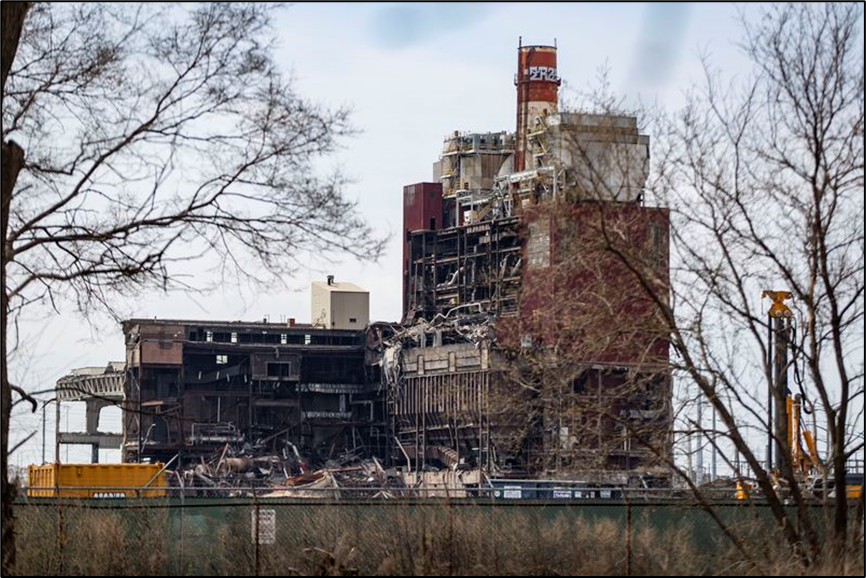
\includegraphics{images/fisk.png}

}

}

\end{minipage}%
%
\begin{minipage}[t]{0.50\linewidth}

{\centering 

\raisebox{-\height}{

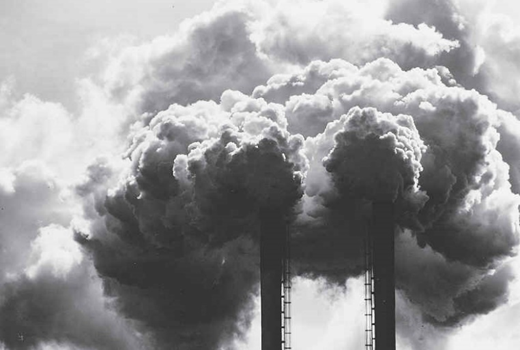
\includegraphics{images/emissions.png}

}

}

\end{minipage}%

\end{figure}

Students will save maps, tables and summaries of spatial analyses in a
\href{https://github.com/justenvirons/pedagogy/raw/main/GEO346_2022_FallQuarter/Exercise_02/Exercise02_AirDispersion_SlidesTemplate.pptx}{PowerPoint
presentation} (or, optionally, a document created with Quarto markdown
in R) to be submitted via the course web page. Students are welcome to
work collectively with classmates to overcome obstacles experienced
while completing the required tasks, although all submissions will be
unique given that students will choose their own study areas that have
different distributions of pollution sources (and therefore different
patterns of air pollutant concentrations). Of course the interpretations
will also be your own. As in all assignments for this class, you will be
asked to not only produce attractive (strive for cartographic
perfection!) and meaningful maps, but also describe patterns presented
within them. The three sections below step you through the process to
create the above deliverable. (For some of the more complicated
procedures, online videos will be made available on the course D2L under
the Exercise \#2 content folder.)

\hypertarget{create-a-new-r-project}{%
\subsection{Create a new R project}\label{create-a-new-r-project}}

In RStudio, create a project within a new directory (e.g.,
GEO336/exercise\_02) of your general course folder. Here you will save
files related to exercise \#2. Create the following folders within the
new exercise-specific directory, ``aermod'', ``data'', ``maps'' and
``scripts''. Install and/or activate the following packages in R using
the below code.

\begin{Shaded}
\begin{Highlighting}[]
\CommentTok{\# install.packages(c("dplyr", "tidyverse", "openxlsx","sf", "sp")) \# uncomment and run if install is necessary}

\FunctionTok{library}\NormalTok{(dplyr) }\CommentTok{\# data wrangling with pipe syntax}
\FunctionTok{library}\NormalTok{(tidyverse) }\CommentTok{\# data wrangling}
\FunctionTok{library}\NormalTok{(openxlsx) }\CommentTok{\# use for importing data in Excel format}
\FunctionTok{library}\NormalTok{(sf) }\CommentTok{\# simple features data package }
\FunctionTok{library}\NormalTok{(sp) }\CommentTok{\# spatial data package}
\end{Highlighting}
\end{Shaded}

\hypertarget{part-two-process-input-data-in-rstudio}{%
\subsection{Part Two: Process input data in
RStudio}\label{part-two-process-input-data-in-rstudio}}

\hypertarget{tri-nei-and-rsei-pollutant-data-for-california}{%
\subsubsection{TRI, NEI and RSEI pollutant data for
California}\label{tri-nei-and-rsei-pollutant-data-for-california}}

Students will draw from two publicly available datasets for this
assignment: NEI and TRI. The
\href{https://www.epa.gov/air-emissions-inventories/national-emissions-inventory-nei}{National
Emissions Inventory} (NEI) is a comprehensive and detailed estimate of
air emissions of criteria pollutants, criteria precursors, and hazardous
air pollutants from air emissions sources. The NEI is released every
three years based primarily upon data provided by State, Local, and
Tribal air agencies for sources in their jurisdictions and supplemented
by data developed by the US EPA. The NEI is built using the Emissions
Inventory System (EIS) first to collect the data from State, Local, and
Tribal air agencies and then to blend that data with other data sources.

The US EPA's
\href{https://www.epa.gov/toxics-release-inventory-tri-program/what-toxics-release-inventory}{Toxics
Release Inventory} (TRI) program tracks the management of certain toxic
chemicals that pose a threat to human health and the environment. Large
US facilities (i.e., those emitting 10 tons or more per year) in
different industry sectors must report annually how much of each
chemical is released to the environment and/or managed through
recycling, energy recovery and treatment. Data containing the 100
most-used data fields from the TRI Reporting Form R and Form A
Certification Statement are made available in various formats on the
\href{https://www.epa.gov/toxics-release-inventory-tri-program/tri-basic-data-files-calendar-years-1987-present}{TRI
Basic Data web page} for reporting years 1987 to 2020. The data can be
downloaded for the entire US or by state.

\begin{Shaded}
\begin{Highlighting}[]
\CommentTok{\# National Emissions Inventory (zip format)}
\NormalTok{temp }\OtherTok{\textless{}{-}} \FunctionTok{tempfile}\NormalTok{()}
\FunctionTok{download.file}\NormalTok{(}\StringTok{"https://gaftp.epa.gov/air/nei/2017/data\_summaries/2017v1/2017neiJan\_facility.zip"}\NormalTok{,temp)}
\NormalTok{NEI\_2017\_raw }\OtherTok{\textless{}{-}} \FunctionTok{read\_csv}\NormalTok{(}\FunctionTok{unz}\NormalTok{(temp, }\StringTok{"emis\_sum\_fac\_15420.csv"}\NormalTok{))}
\FunctionTok{unlink}\NormalTok{(temp)}

\CommentTok{\# format NEI data}
\CommentTok{\# filter sulfur dioxide releases in California}
\NormalTok{NEI\_2017\_form }\OtherTok{\textless{}{-}}\NormalTok{ NEI\_2017\_raw }\SpecialCharTok{\%\textgreater{}\%}
  \FunctionTok{rename}\NormalTok{(}
    \AttributeTok{fac\_name =} \StringTok{\textasciigrave{}}\AttributeTok{company name}\StringTok{\textasciigrave{}}\NormalTok{,}
    \AttributeTok{site\_name =} \StringTok{\textasciigrave{}}\AttributeTok{site name}\StringTok{\textasciigrave{}}\NormalTok{,}
    \AttributeTok{fac\_street =}\NormalTok{ address,}
    \AttributeTok{fac\_city =}\NormalTok{ city,}
    \AttributeTok{fac\_state =} \StringTok{\textasciigrave{}}\AttributeTok{postal abbreviation}\StringTok{\textasciigrave{}}\NormalTok{,}
    \AttributeTok{fac\_zip =} \StringTok{\textasciigrave{}}\AttributeTok{zip code}\StringTok{\textasciigrave{}}\NormalTok{,}
    \AttributeTok{naics\_code =} \StringTok{\textasciigrave{}}\AttributeTok{naics code}\StringTok{\textasciigrave{}}\NormalTok{,}
    \AttributeTok{naics\_desc =} \StringTok{\textasciigrave{}}\AttributeTok{naics description}\StringTok{\textasciigrave{}}\NormalTok{,}
    \AttributeTok{latitude =} \StringTok{\textasciigrave{}}\AttributeTok{site latitude}\StringTok{\textasciigrave{}}\NormalTok{,}
    \AttributeTok{longitude =} \StringTok{\textasciigrave{}}\AttributeTok{site longitude}\StringTok{\textasciigrave{}}\NormalTok{,}
    \AttributeTok{pollutant\_code =} \StringTok{\textasciigrave{}}\AttributeTok{pollutant code}\StringTok{\textasciigrave{}}\NormalTok{,}
    \AttributeTok{pollutant\_desc =} \StringTok{\textasciigrave{}}\AttributeTok{pollutant desc}\StringTok{\textasciigrave{}}\NormalTok{,}
    \AttributeTok{pollutant\_type =} \StringTok{\textasciigrave{}}\AttributeTok{pollutant type(s)}\StringTok{\textasciigrave{}}\NormalTok{,}
    \AttributeTok{emissions\_uom =} \StringTok{\textasciigrave{}}\AttributeTok{emissions uom}\StringTok{\textasciigrave{}}\NormalTok{,}
    \AttributeTok{emissions =} \StringTok{\textasciigrave{}}\AttributeTok{total emissions}\StringTok{\textasciigrave{}}
\NormalTok{  ) }\SpecialCharTok{\%\textgreater{}\%}
  \FunctionTok{select}\NormalTok{(}
\NormalTok{    fac\_name,}
\NormalTok{    site\_name,}
\NormalTok{    fac\_street,}
\NormalTok{    fac\_city,}
\NormalTok{    fac\_state,}
\NormalTok{    fac\_zip,}
\NormalTok{    naics\_code,}
\NormalTok{    naics\_desc,}
\NormalTok{    latitude,}
\NormalTok{    longitude,}
\NormalTok{    pollutant\_code,}
\NormalTok{    pollutant\_desc,}
\NormalTok{    pollutant\_type,}
\NormalTok{    emissions\_uom,}
\NormalTok{    emissions}
\NormalTok{  ) }\SpecialCharTok{\%\textgreater{}\%}
  \FunctionTok{filter}\NormalTok{(fac\_state }\SpecialCharTok{==} \StringTok{"CA"}\NormalTok{,}
\NormalTok{         pollutant\_code }\SpecialCharTok{==} \StringTok{"SO2"}\NormalTok{)}

\CommentTok{\# Toxics Release Inventory (csv format)}
\NormalTok{TRI\_2020\_raw }\OtherTok{\textless{}{-}} \FunctionTok{read\_csv}\NormalTok{(}\StringTok{"https://enviro.epa.gov/enviro/efservice/MV\_TRI\_BASIC\_DOWNLOAD/year/=/2020/fname/TRI\_2020\_US.csv/CSV?.csv"}\NormalTok{)}

\CommentTok{\# format TRI data}
\CommentTok{\# filter data stack air releases in California}
\NormalTok{TRI\_2020\_form }\OtherTok{\textless{}{-}}\NormalTok{ TRI\_2020\_raw }\SpecialCharTok{\%\textgreater{}\%}
  \FunctionTok{rename}\NormalTok{(}
    \AttributeTok{year =} \DecValTok{1}\NormalTok{,}
    \AttributeTok{fac\_name =} \DecValTok{4}\NormalTok{,}
    \AttributeTok{fac\_street =} \DecValTok{5}\NormalTok{,}
    \AttributeTok{fac\_city =} \DecValTok{6}\NormalTok{,}
    \AttributeTok{fac\_county =} \DecValTok{7}\NormalTok{,}
    \AttributeTok{fac\_state =} \DecValTok{8}\NormalTok{,}
    \AttributeTok{fac\_zip =} \DecValTok{9}\NormalTok{,}
    \AttributeTok{latitude =} \DecValTok{12}\NormalTok{,}
    \AttributeTok{longitude =} \DecValTok{13}\NormalTok{,}
    \AttributeTok{parent\_co =} \DecValTok{15}\NormalTok{,}
    \AttributeTok{sector\_code =} \DecValTok{19}\NormalTok{,}
    \AttributeTok{sector\_name =} \DecValTok{20}\NormalTok{,}
    \AttributeTok{chemical =} \DecValTok{34}\NormalTok{,}
    \AttributeTok{casno =} \DecValTok{37}\NormalTok{,}
    \AttributeTok{srsid =} \DecValTok{38}\NormalTok{,}
    \AttributeTok{caa\_chemical =} \DecValTok{39}\NormalTok{,}
    \AttributeTok{carcinogen =} \DecValTok{43}\NormalTok{,}
    \AttributeTok{pfas =} \DecValTok{44}\NormalTok{,}
    \AttributeTok{emissions\_uom =} \DecValTok{46}\NormalTok{,}
    \AttributeTok{fugitive\_air =} \DecValTok{47}\NormalTok{,}
    \AttributeTok{stack\_air =} \DecValTok{48}\NormalTok{,}
    \AttributeTok{water =} \DecValTok{49}\NormalTok{,}
    \AttributeTok{underground =} \DecValTok{50}
\NormalTok{  ) }\SpecialCharTok{\%\textgreater{}\%}
  \FunctionTok{select}\NormalTok{(}
\NormalTok{    year,}
\NormalTok{    fac\_name,}
\NormalTok{    fac\_street,}
\NormalTok{    fac\_city,}
\NormalTok{    fac\_county,}
\NormalTok{    fac\_state,}
\NormalTok{    fac\_zip,}
\NormalTok{    latitude,}
\NormalTok{    longitude,}
\NormalTok{    parent\_co,}
\NormalTok{    sector\_code,}
\NormalTok{    sector\_name,}
\NormalTok{    chemical,}
\NormalTok{    casno,}
\NormalTok{    srsid,}
\NormalTok{    caa\_chemical,}
\NormalTok{    carcinogen,}
\NormalTok{    pfas,}
\NormalTok{    emissions\_uom,}
\NormalTok{    fugitive\_air,}
\NormalTok{    stack\_air,}
\NormalTok{    water,}
\NormalTok{    underground}
\NormalTok{  ) }\SpecialCharTok{\%\textgreater{}\%}
  \FunctionTok{filter}\NormalTok{(fac\_state }\SpecialCharTok{==} \StringTok{"CA"}\NormalTok{,}
\NormalTok{         stack\_air }\SpecialCharTok{\textgreater{}} \DecValTok{0}\NormalTok{)}

\CommentTok{\# RSEI data (Excel format)}
\NormalTok{RSEI\_v2310\_raw }\OtherTok{\textless{}{-}} \FunctionTok{read.xlsx}\NormalTok{(}\StringTok{"https://www.epa.gov/system/files/other{-}files/2022{-}02/toxicity\_data\_rsei\_v2310.xlsx"}\NormalTok{, }\AttributeTok{sheet=}\DecValTok{2}\NormalTok{)}

\NormalTok{RSEI\_v2310\_form }\OtherTok{\textless{}{-}}\NormalTok{ RSEI\_v2310\_raw }\SpecialCharTok{\%\textgreater{}\%}
  \FunctionTok{rename}\NormalTok{(}\AttributeTok{casno =}\NormalTok{ CASStandard) }\SpecialCharTok{\%\textgreater{}\%}
  \FunctionTok{mutate}\NormalTok{(}\AttributeTok{itw =} \FunctionTok{as.numeric}\NormalTok{(ITW)) }\SpecialCharTok{\%\textgreater{}\%}
  \FunctionTok{select}\NormalTok{(casno, }
\NormalTok{         itw)}
\end{Highlighting}
\end{Shaded}

EPA's Risk-Screening Environmental Indicators (RSEI) model helps policy
makers, researchers, and communities explore data on releases of toxic
substances from industrial and federal facilities. The model considers
the fate and transport of chemicals through the environment, each
chemical's relative toxicity, and potential human exposure. When
combined with the total releases of chemicals by location, RSEI model
results can be used to help identify locations of toxic hot spots,
monitor potential human health impacts over time, prioritize
investigative work and prioritize the allocation of agency resources,
more generally. Use the following code to join RSEI toxicity weights to
the TRI data.

\begin{Shaded}
\begin{Highlighting}[]
\CommentTok{\# Join TRI with RSEI inhalation toxicity weights (ITW)}
\NormalTok{TRI\_2020\_form\_wtd }\OtherTok{\textless{}{-}}\NormalTok{ TRI\_2020\_form }\SpecialCharTok{\%\textgreater{}\%} 
  \FunctionTok{left\_join}\NormalTok{(RSEI\_v2310\_form, }\AttributeTok{by =} \StringTok{"casno"}\NormalTok{) }\SpecialCharTok{\%\textgreater{}\%}
  \FunctionTok{mutate}\NormalTok{(}\AttributeTok{stack\_air\_itw =}\NormalTok{ stack\_air }\SpecialCharTok{*}\NormalTok{ itw}\SpecialCharTok{/}\DecValTok{10000000}\NormalTok{) }\SpecialCharTok{\%\textgreater{}\%}
  \FunctionTok{drop\_na}\NormalTok{(stack\_air\_itw) }\SpecialCharTok{\%\textgreater{}\%}
  \FunctionTok{select}\NormalTok{(}\SpecialCharTok{{-}}\NormalTok{itw)}
\end{Highlighting}
\end{Shaded}

\hypertarget{create-and-write-shapefiles}{%
\subsubsection{Create and write
shapefiles}\label{create-and-write-shapefiles}}

Save the NEI and TRI air pollution tables as shapefiles into your
working directory, perhaps in the ``data'' folder. If you are choosing
to examine an area located within northern California, use UTM 10N
(EPSG: 26910) and UTM 11N (EPSG: 26911) if your study area is in
southern California. See a general map of the UTM zones for the
contiguous United States below.

\includegraphics{images/fig44.gif}

\begin{Shaded}
\begin{Highlighting}[]
\NormalTok{TRI\_2020\_form\_wtd\_geom }\OtherTok{\textless{}{-}} \FunctionTok{st\_as\_sf}\NormalTok{(TRI\_2020\_form\_wtd, }\AttributeTok{coords =} \FunctionTok{c}\NormalTok{(}\StringTok{"longitude"}\NormalTok{, }\StringTok{"latitude"}\NormalTok{), }\AttributeTok{crs =} \DecValTok{4269}\NormalTok{) }\SpecialCharTok{\%\textgreater{}\%} \FunctionTok{st\_transform}\NormalTok{(}\AttributeTok{crs=}\DecValTok{26911}\NormalTok{) }\SpecialCharTok{\%\textgreater{}\%}
  \FunctionTok{st\_as\_sf}\NormalTok{() }\CommentTok{\# or crs = 26910 if in northern California}

\FunctionTok{st\_write}\NormalTok{(TRI\_2020\_form\_wtd\_geom, }\StringTok{"enter working directory and desired file name"}\NormalTok{,}\AttributeTok{append=}\ConstantTok{FALSE}\NormalTok{)}

\NormalTok{NEI\_2017\_form\_geom }\OtherTok{\textless{}{-}} \FunctionTok{st\_as\_sf}\NormalTok{(NEI\_2017\_form, }\AttributeTok{coords =} \FunctionTok{c}\NormalTok{(}\StringTok{"longitude"}\NormalTok{, }\StringTok{"latitude"}\NormalTok{), }\AttributeTok{crs =} \DecValTok{4269}\NormalTok{) }\SpecialCharTok{\%\textgreater{}\%} \FunctionTok{st\_transform}\NormalTok{(}\AttributeTok{crs=}\DecValTok{26911}\NormalTok{) }\SpecialCharTok{\%\textgreater{}\%}
  \FunctionTok{st\_as\_sf}\NormalTok{() }\CommentTok{\# or crs = 26910 if in northern California}

\FunctionTok{st\_write}\NormalTok{(NEI\_2017\_form\_geom, }\StringTok{"enter working directory and desired file name"}\NormalTok{,}\AttributeTok{append=}\ConstantTok{FALSE}\NormalTok{)}
\end{Highlighting}
\end{Shaded}

\hypertarget{part-three-create-and-add-data-to-arcgis-pro-project}{%
\subsection{Part Three: Create and add data to ArcGIS Pro
project}\label{part-three-create-and-add-data-to-arcgis-pro-project}}

\hypertarget{add-and-download-spatial-data}{%
\subsubsection{Add and download spatial
data}\label{add-and-download-spatial-data}}

Create a new ArcGIS Pro project on your computer under the maps
directory in your R project folder. In your ArcGIS Pro map project,
under the ``Map'' menu, click the ``Add Data'' option on the toolbar and
navigate to the directory where you exported the NEI and TRI datasets.
You may need to click the ``Connect to Folder'' and navigate to your
project directory. Select all three of the files and add to the map
frame. They should draw automatically and appear in the table of
contents.

Also download the
\href{https://ww3.arb.ca.gov/ei/gislib/boundaries/ca_co_ab_dis.zip}{California
county, air basin and air district boundary file} from the
\href{https://ww2.arb.ca.gov/geographical-information-system-gis-library}{California
Air Resources Board (CARB) GIS Library web page}. These boundaries will
be helpful to identify the entity that provides AERMOD-ready
meteorological data given that AERMOD requires such data to estimate the
geographic distribution of releases over time.

\begin{tcolorbox}[enhanced jigsaw, colbacktitle=quarto-callout-note-color!10!white, rightrule=.15mm, title=\textcolor{quarto-callout-note-color}{\faInfo}\hspace{0.5em}{Meteorological data}, bottomrule=.15mm, opacityback=0, bottomtitle=1mm, leftrule=.75mm, opacitybacktitle=0.6, colframe=quarto-callout-note-color-frame, titlerule=0mm, left=2mm, toprule=.15mm, breakable, arc=.35mm, colback=white, toptitle=1mm, coltitle=black]
The California Air Resources Board (CARB) makes available
\href{https://ww2.arb.ca.gov/resources/documents/harp-aermod-meteorological-files}{AERMOD-ready
meteorological data for 28 select weather stations throughout the state}
while the various air quality districts make available similarly
formatted data for weather stations within their respective
jurisdictions. Links to the district-specific weather station and data
are also available on the
\href{https://ww2.arb.ca.gov/resources/documents/harp-aermod-meteorological-files}{ARB
meteorological data webpage}.
\end{tcolorbox}

\hypertarget{part-four-create-study-area}{%
\subsection{Part Four: Create Study
Area}\label{part-four-create-study-area}}

You will need to create a custom and spatially explicit study area in
order to run the needed calculations. Create your custom study area by
doing the following:

\begin{itemize}
\item
  Under the ``View'' menu, click the ``Catalog Pane'' option to view
  project contents. Navigate to your project folder and right-click on
  the ``Data'' directory to create a new shapefile. With your project
  directory selected, open the File menu and select the
  ``New/Shapefile'' option. In the ``Create Feature Class'' dialog box,
  give your polygonal shapefile an appropriate name (e.g., studyarea).
  Be sure the output coordinate system corresponds with the other
  shapefiles in your map frame (i.e., UTM Zone 10N, NAD 1983). When
  finished, add the new shapefile to the map.

  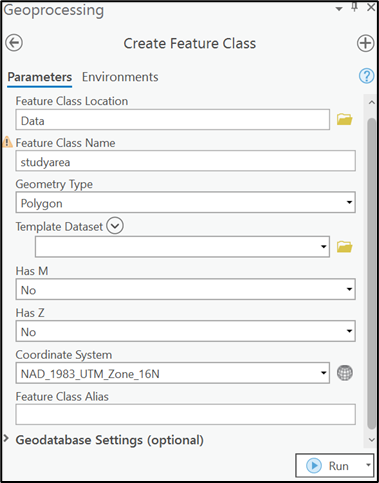
\includegraphics[width=3in,height=\textheight]{images/paste-D249D986.png}
\item
  In the ``Edit'' menu, click ``Create'' to begin delineating the study
  area polygon. In the ``Create Features'' dialog, use the square
  template to construct the polygon. With the pencil tool activated,
  create a 10km by 10km square by clicking the map to create the initial
  vertex. Don't be concerned about the specific location of the initial
  vertex (and study area) at this time. While still editing, right-click
  inside the map frame and select the ``Direction/Size'' option to make
  visible the associated dialog box. Enter ``0'' for direction and 10km
  for both length and width. When finished entering the dimensions click
  the Enter key on your keyboard to create the new feature.

  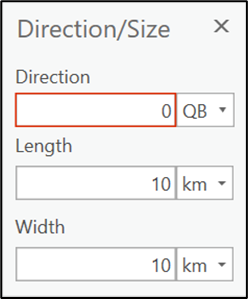
\includegraphics[width=1.5in,height=\textheight]{images/paste-F8F29155.png}
\end{itemize}

\hypertarget{part-five-model-facility-and-cumulative-impact-of-criteria-air-emissions-so2}{%
\subsection{Part Five: Model facility and cumulative impact of criteria
air emissions
(SO2)}\label{part-five-model-facility-and-cumulative-impact-of-criteria-air-emissions-so2}}

In this part of the exercise you will analyze the concentrations of
sulfur dioxide emitted from a specific facility and then compare this
with the cumulative sulfur dioxide emissions (from all facilities)
within (and/or near) your study area.

\begin{itemize}
\item
  First, identify a single facility in the NEI facilities shapefile that
  emits considerable amounts of sulfur dioxide (SO2).
\item
  Next, center the study area so that the facility you identified is
  located in the (approximate) center. Do this by clicking on the
  ``Edit'' menu and selecting the study area polygon. Use the ``Move''
  tool to position the polygon in the desired location. Under the
  ``Share'' menu, click ``Capture to Clipboard'' and paste the NEI
  facilities map into the appropriate PowerPoint slide.

  \begin{figure}

  {\centering 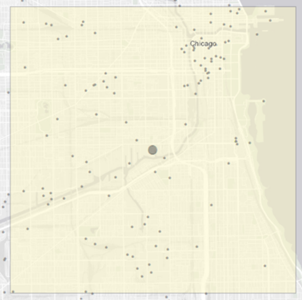
\includegraphics[width=2in,height=\textheight]{images/paste-8B95D98A.png}

  }

  \caption{``10kmx10km study area with facilities mappeed by annual SO2
  emissions (tons)''}

  \end{figure}
\end{itemize}

Now you will use AERMOD to model emissions from the facility you
selected. Read through the AERMOD Primer in Appendix C before
proceeding.

\begin{itemize}
\item
  Using a text editor (such as notepad or my preference is notetab light
  freeware), edit aermod.inp so that the source (SO LOCATION) pathway
  location coordinates (X and Y) reflect those of your selected facility
  and the source (SO SRCPARAM) parameters reflect the SO2 emissions from
  the selected facility in the proper units (grams per second). Convert
  the tons per year to grams per second using the
  \href{https://github.com/justenvirons/pedagogy/raw/main/GEO346_2022_FallQuarter/Exercise_02/aermod/AERMODFormatting.xls}{AERMOD\_Formatting.xlsx}
  spreadsheet which uses the following formula: quantity in g/s =
  (tons/year*2000 pounds/year*453.59237 grams/pound)/(365 days/year * 24
  hrs/day * 60 minutes/hour * 60 seconds/minute)). Use the default
  (i.e., existing) settings for the release height, stack gas exit
  temperature, stack gas exit velocity, and stack diameter (e.g., 76.
  353. 5. 3.0) for the facility.
\item
  Also edit in aermod.inp the receptor (or RE) pathway so that the
  bottom, left (southwest vertex in this case) coordinates (the anchor
  point of the Cartesian grid) reflect those of your study area (you can
  identify coordinates via the status bar at the bottom right of the
  ArcGIS Pro map frame or via the Properties/Source/Extent menu by
  right-clicking on feature layer). Use the existing 200m x 50m
  parameters for the Cartesian receptor grid (e.g., XYINC 50 {[}bottom
  left X coordinate of study area{]} and 200 {[}bottom left Y coordinate
  of study area{]}). You can again use the
  \href{https://github.com/justenvirons/pedagogy/raw/main/GEO346_2022_FallQuarter/Exercise_02/aermod/AERMODFormatting.xls}{AERMODFormatting.xlsx}
  spreadsheet to format this parameter for the aermod.inp file.
\item
  Note that we may need to reduce processing time by calculating
  concentrations for fewer days than what is available in the
  meteorology files. If it takes too long for your machine to calculate
  over multiple years it may be necessary to spread the analysis across
  a select number of days over different months for a single year in
  order to account for seasonal variations (1/1-1/7; 4/1-4/7; 10/1-10/7;
  7/1-7/7). Be sure that the meteorological (ME) pathway refers to the
  meteorological files for the entire study period/year.
\item
  Next set the output (OU) pathway to create four plot files, with each
  representing key concentrations over given periods of time. The
  default input file calculates maximum concentrations averaged over
  one- and three-hour periods. Concentrations will be estimated for each
  of the 2,500 receptors in your study area. Also rename the output plot
  files in the OU parameters so they are more informative (e.g.,
  NEI\_3HRMAX.PLT, NEI\_1HRMAX.PLT).
\item
  Now you are ready to run the newly specified model. To run the model,
  navigate to the directory where aermod.inp, aermod.exe and the
  associated meteorological files are located. Double-click the
  aermod.exe executable file (or drag and release aermod.inp over
  aermod.exe). Allow AERMOD to cycle through the 365 days of the year.
  If you receive an error, check the sources of the error by reading the
  ERROR.OUT file in notepad or other text editor.
\item
  Once AERMOD has completed the procedure, you will need to re-format
  the data in the plot file so that it is readable in ArcGIS Pro. First,
  open the 1-hour maximum concentrations plot file in notepad (under the
  ``Format'' menu, be sure the word wrap is off, not checked). Remove
  much of the header documentation, remove spaces in column names in the
  plot file so that it appears as follows. Save the edited plot file.

  \begin{figure}

  {\centering 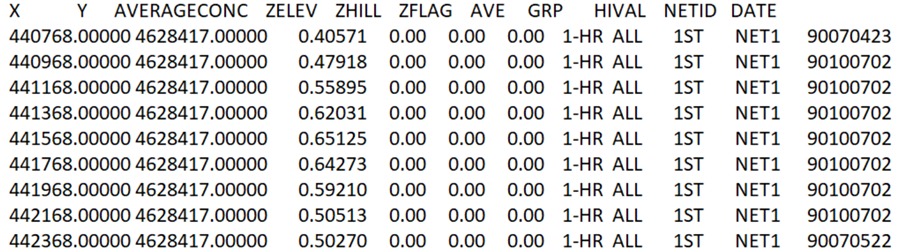
\includegraphics{images/paste-B5992985.png}

  }

  \caption{Sample of AERMOD output file}

  \end{figure}
\item
  Next, open the plot file in Excel using the default fixed width
  settings. Remove any spaces and parentheses from the column names
  (ArcGIS Pro only allows numbers, characters and underscores in field
  names). Save the text file as a CSV file. Also be sure to close the
  file in Excel before attempting to open it in ArcGIS Pro.
\item
  Return to ArcGIS Pro and open the annual, comma delimited text file.
  In order to display the model output, click the ``Add Data'' option in
  the ``Map'' menu and select the ``XY Point Data'' option. ArcGIS Pro
  will open a ``XY Table to Point'' dialog. Navigate to the input CSV
  table you just created. ArcGIS Pro should automatically recognize the
  X and Y fields in the input file. Specify the output location and
  feature class as a layer in the project geodatabase (``.shp'' suffix).
  Edit the coordinate system information so that it corresponds with the
  other shapefiles in the map frame (e.g., UTM Zone 11N, NAD 1983). When
  finished, click ``Run'' and the new point layer should be added to the
  map table of contents. Make visible the layer to show the series of
  receptor points specified in the AERMOD input file. Next, open the
  plot file in Excel using the default fixed width settings. Remove any
  spaces and parentheses from the column names (ArcGIS Pro only allows
  numbers, characters and underscores in field names). Save the text
  file as a CSV file. Also be sure to close the file in Excel before
  attempting to open it in ArcGIS Pro.
\item
  Return to ArcGIS Pro and open the annual, tab-delimited text file. In
  order to display the model output, click the ``Add Data'' option in
  the ``Map'' menu and select the ``XY Point Data'' option. ArcGIS Pro
  will open a ``XY Table to Point'' dialog. Navigate to the input CSV
  table you just created. ArcGIS Pro should automatically recognize the
  X and Y fields in the input file. Specify the output location and
  feature class as a layer in the project geodatabase (``.shp'' suffix).
  Edit the coordinate system information so that it corresponds with the
  other shapefiles in the map frame (i.e., UTM Zone 11N, NAD 1983). When
  finished, click ``Run'' and the new point layer should be added to the
  map table of contents. Make visible the layer to show the series of
  receptor points specified in the AERMOD input file.

  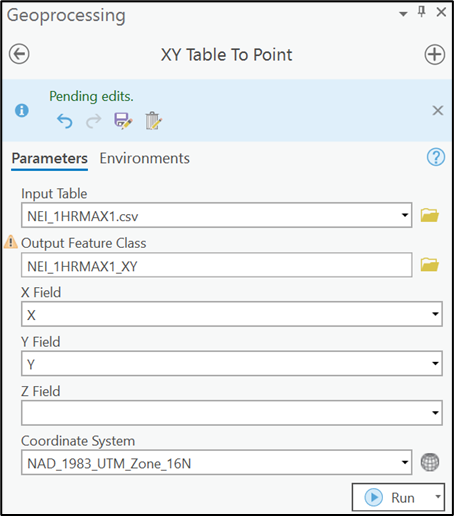
\includegraphics[width=2.5in,height=\textheight]{images/paste-24DE3A0C.png}
\item
  In order to better display variations in concentrations within your
  study area, convert the points to grid cells. Do this by clicking the
  ``Tools'' option under the ``Analysis'' menu. In the ``Geoprocessing''
  dialog, type ``Point to Raster'' to open the associated conversion
  tool. Specify the output cell size as 200 (to correspond with the
  parameters specified in the AERMOD input file) and click Run when
  finished. Create a histogram to show the distributions of values
  within the raster layer, including the mean, median and standard
  deviation. Copy and paste the 1-hour maximum concentration map, legend
  and histogram into the appropriate slide within the
  \href{https://github.com/justenvirons/pedagogy/raw/main/GEO346_2022_FallQuarter/Exercise_02/Exercise02_AirDispersion_SlidesTemplate.pptx}{PowerPoint
  template}. Also, view the ``metadata'' tab on the Properties dialog
  for the raster layer to view statistics for the concentrations field.
  Populate the appropriate column in the PowerPoint table template
  (Slide 5) with corresponding values.

  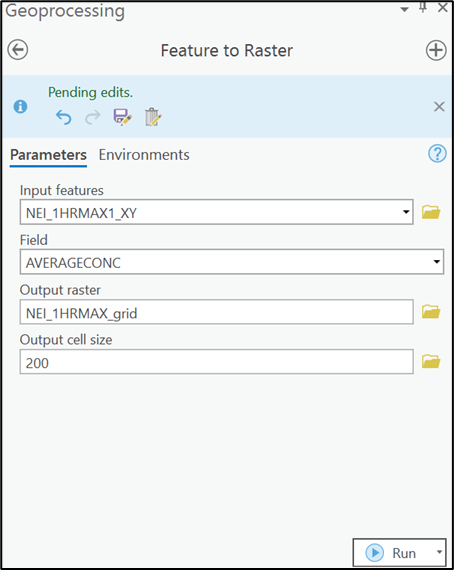
\includegraphics[width=2.5in,height=\textheight]{images/paste-C52CEE31.png}
\item
  Repeat the above three procedures to map the 3-hour concentration plot
  for the single facility. To complete the remaining maps for part two,
  refer to the above steps to calculate SO2 emissions from multiple
  facilities within your study area. For the multiple facilities (or
  cumulative analysis), begin by selecting all facilities inside and
  within one kilometer of your study area (hint: use the buffer distance
  option under the ``select by location'' option under the ``Select''
  menu). Open the attribute table with selected facilities that emit
  criteria pollutants. Use the export tool to save selected records in
  dbf format. Open the dBase file in Excel. In Excel sort the facilities
  to identify the top five emitters of SO2 and use the provided
  AERMODFormatting.xls spreadsheet to format source location and source
  parameter specifications for the five AERMOD facilities.
\item
  Lastly compare the modeled pollutant concentrations in your study area
  to the regulatory reference concentrations (Appendix A provides US EPA
  national air quality standards by concentration category; i.e., 1hr
  and 3-hour) and write-up your findings. In your write-up, respond to
  questions concerning the degree to which the facility contributes to
  pollutant concentrations within the study area. Also consider any
  limitations or concerns you may have about the model (e.g., what is
  excluded from the model).
\end{itemize}

\hypertarget{part-six-model-seasonal-variation-in-toxic-air-concentrations}{%
\subsection{Part Six: Model seasonal variation in toxic air
concentrations}\label{part-six-model-seasonal-variation-in-toxic-air-concentrations}}

Air toxics, unlike ``criteria'' air pollutants such as ground-level
ozone and oxides of nitrogen whose main health impact is their
contribution to smog, are more localized in their impact. These
substances can contribute to risk of cancer, respiratory illness, and
other harms when inhaled. Their unequal distribution across the country
and even within communities has often not been remedied successfully
even as the Clean Air Act has been relatively successful at cleaning
criteria pollutants from the air.

In this part of the exercise, you will estimate toxic air releases
within your study area from large, industrial facilities represented in
the latest (2020) EPA's Toxics Release Inventory or TRI report. The TRI
reports emissions by facility for each of the 650 toxics and toxic
compounds. Given that every chemical has a different dose-response curve
or, more simply, a different toxicological profile, you will adjust
chemical releases using inhalation toxicity weighted factors (ITW) from
EPA's Risk-Screening Environmental Indicators (RSEI) model. The
toxicity-weighted concentrations are provided are an appropriate metric
for comparing levels of potential impact between geographic areas and
for smaller-scale environmental justice analyses. Further,
toxicity-weighted allows concentrations to be added across chemicals for
the same geographic area.

For Part Six, you will explore only the maximum 3-hour concentration
plot files for the inhalation toxicity weighted (ITW) emissions arising
from all facilities within the study area (select multiple facilities
using the same procedure used above).

You will alter parameters in the (ME) pathway in order to estimate how
the distribution of air concentrations differs seasonally due to changes
in wind direction, wind speed and air temperature. This said, you will
run four AERMOD models; one for each season. In order to run the
season-specific models, change the meteorological pathway (ME)
parameters so that it references the appropriate season-specific upper
air and surface files (e.g., we will go over the seasonal date ranges in
class). As before, for the multiple facilities (or cumulative analysis),
select the five facilities within the study area with the highest ITW
concentrations. Use the AERMODFormatting.xls spreadsheet to format data
for AERMOD input files. Create associated maps and update the
corresponding table (Slide 10). Summarize your findings in the write-up
for (Slide 11).

\hypertarget{refs}{}
\begin{CSLReferences}{1}{0}
\leavevmode\vadjust pre{\hypertarget{ref-ala2022}{}}%
ALA. 2022. {``State of the {Air} 202.''} {Chicago, IL}: {American Lung
Association}.

\leavevmode\vadjust pre{\hypertarget{ref-ard2020}{}}%
Ard, Kerry, and Clair Bullock. 2020. {``Chapter 12 - {Concentrating}
Risk? {The} Geographic Concentration of Health Risk from Industrial Air
Toxics Across {America}.''} In \emph{Spatiotemporal {Analysis} of {Air
Pollution} and {Its Application} in {Public Health}}, edited by Lixin
Li, Xiaolu Zhou, and Weitian Tong, 277--92. {Elsevier}.
\url{https://doi.org/10.1016/B978-0-12-815822-7.00012-1}.

\leavevmode\vadjust pre{\hypertarget{ref-usepa2014}{}}%
EPA, US. 2014. {``{NAAQS Table}.''} Other \{\{Policies\}\} and
\{\{Guidance\}\}.
https://www.epa.gov/criteria-air-pollutants/naaqs-table.

\leavevmode\vadjust pre{\hypertarget{ref-landrigan2017}{}}%
Landrigan, Philip J. 2017. {``Air Pollution and Health.''} \emph{The
Lancet Public Health} 2 (1): e4--5.
\url{https://doi.org/10.1016/S2468-2667(16)30023-8}.

\leavevmode\vadjust pre{\hypertarget{ref-lejano2006b}{}}%
Lejano, Raul P., and C. Scott Smith. 2006. {``Incompatible {Land Uses}
and the {Topology} of {Cumulative Risk}.''} \emph{Environmental
Management} 37 (2): 230--46.

\leavevmode\vadjust pre{\hypertarget{ref-usepa2013}{}}%
US EPA, OP. 2013. {``Summary of the {Clean Air Act}.''} Overviews and
\{\{Factsheets\}\}.
https://www.epa.gov/laws-regulations/summary-clean-air-act.

\end{CSLReferences}



\end{document}
